\documentclass{article}
\usepackage[utf8]{inputenc}
\usepackage[english]{babel}
\usepackage {graphicx}
\usepackage{amsmath}

\begin{document}
	\author{Michael Gabler (2381427), Matthias Clad (2349277)}
	\title{Robotics 1 - Exercise 11}
	\date{09.01.2018}
	\maketitle
	
	\newpage
	
	\tableofcontents
	
	\newpage
	
	\section{Task 3.1}
	\paragraph{Proof for $\varphi = \arctan(\frac{\tan \varphi_{r}}{1-\frac{d}{2l}\tan \varphi_{r}})$}
	
	\begin{gather}
	\tan \varphi = \frac{l}{r}
	\Leftrightarrow
	r = \frac{l}{\tan \varphi}
	\end{gather}
	\begin{gather}
	\nonumber \tan \varphi_{r} = \frac{l}{r + \frac{d}{2}} \Rightarrow 
	\tan \varphi_{r} = \frac{l}{\frac{l}{\tan \varphi} + \frac{d}{2}} = \tan \varphi + \frac{2l}{d}
	\Leftrightarrow\\
	\nonumber \tan \varphi = \tan \varphi_{r} - \frac{2l}{d} = (1 - \frac{2l}{d \tan \varphi_{r}}) \tan \varphi_{r} = \frac{\tan \varphi_{r}}{1 - \frac{d}{2l} \tan \varphi_{r}}
	\Leftrightarrow\\
	\varphi = \arctan(\frac{\tan \varphi_{r}}{1-\frac{d}{2l}\tan \varphi_{r}})
	\end{gather}
	
	\paragraph{Proof for $\varphi = \arctan(\frac{\tan \varphi_{l}}{1+\frac{d}{2l}\tan \varphi_{l}})$}
	
	\begin{gather}
	\nonumber \tan \varphi_{l} = \frac{l}{r - \frac{d}{2}} \Rightarrow 
	\tan \varphi_{l} = \frac{l}{\frac{l}{\tan \varphi} - \frac{d}{2}} = \tan \varphi - \frac{2l}{d}
	\Leftrightarrow\\
	\nonumber \tan \varphi = \tan \varphi_{l} + \frac{2l}{d} = (1 + \frac{2l}{d \tan \varphi_{l}}) \tan \varphi_{l} = \frac{\tan \varphi_{l}}{1 + \frac{d}{2l} \tan \varphi_{l}}
	\Leftrightarrow\\
	\varphi = \arctan(\frac{\tan \varphi_{l}}{1+\frac{d}{2l}\tan \varphi_{l}})
	\end{gather}
	

	\section{Task 3.2}
	\paragraph{Differential-drive robot}
	
	\begin{gather}
	\Delta \theta = \theta(t_{2}) - \theta(t_{1}) = \int_{t_{1}}^{t_{2}} \dot{\theta}(t) dt = \int_{t_{1}}^{t_{2}} \frac{1}{d} (v_{r} - v_{l}) dt = \frac{t_{2} - t_{1}}{d} (v_{r} - v_{l})
	\end{gather}
	\begin{gather}
	\nonumber \Delta x = x(t_{2}) - x(t_{1}) = \int_{t_{1}}^{t_{2}} \dot{x}(t) dt = \int_{t_{1}}^{t_{2}} \frac{1}{2} \cos(\theta(t)) (v_{r} + v_{l}) dt =\\
	\nonumber \frac{1}{2 \dot{\theta}(t_{2})} \sin(\theta(t_{2})) (v_{r} + v_{l}) - \frac{1}{2 \dot{\theta}(t_{1})} \sin(\theta(t_{1})) (v_{r} + v_{l}) =\\
	\frac{d(v_{r} + v_{l})}{2(v_{r} - v_{l})}(\sin(\frac{t_{2}}{d}(v_{r} - v_{l})) - \sin(\frac{t_{1}}{d}(v_{r} - v_{l})))
	\end{gather}
	\begin{gather}
	\nonumber \Delta y = y(t_{2}) - y(t_{1}) = \int_{t_{1}}^{t_{2}} \dot{y}(t) dt = \int_{t_{1}}^{t_{2}} \frac{1}{2} \sin(\theta(t)) (v_{r} + v_{l}) dt =\\
	\nonumber -\frac{1}{2 \dot{\theta}(t_{2})} \cos(\theta(t_{2})) (v_{r} + v_{l}) + \frac{1}{2 \dot{\theta}(t_{1})} \cos(\theta(t_{1})) (v_{r} + v_{l}) =\\
	-\frac{d(v_{r} + v_{l})}{2(v_{r} - v_{l})}(\cos(\frac{t_{2}}{d}(v_{r} - v_{l})) - \cos(\frac{t_{1}}{d}(v_{r} - v_{l})))
	\end{gather}
	
	The equations can't be used for straight line motion. $\theta(t)$ and $\dot{\theta}(t)$ will be 0 for each $t$ because $v_{r}$ and $v_{l}$ are equal for straight line motion. Then there's a division by 0 when calculating $x(t)$ and $y(t)$.\\
	
	With $v_{r} = v_{l}$:
	\begin{gather}
	\dot{p} = 
	\begin{bmatrix}
	\dot{x}(t)\\
	\dot{y}(t)\\
	\dot{\theta}(t)
	\end{bmatrix} = 
	\begin{bmatrix}
	1\\
	0\\
	0
	\end{bmatrix} v(t)\\
	v(t) = \frac{1}{2}(v_{r} + v_{l})
	\end{gather}
	
	\paragraph{Car-like robot}
	\begin{gather}
	\Delta \theta = \theta(t_{2}) - \theta(t_{1}) = \int_{t_{1}}^{t_{2}} \dot{\theta}(t) dt = \int_{t_{1}}^{t_{2}} \frac{\tan \varphi}{l} v dt = \frac{\tan \varphi}{l} v (t_{2} - t_{1})
	\end{gather}
	\begin{gather}
	\nonumber \Delta x = x(t_{2}) - x(t_{1}) = \int_{t_{1}}^{t_{2}} \dot{x}(t) dt = \int_{t_{1}}^{t_{2}} \cos(\theta(t)) v dt =\\
	\nonumber \frac{v}{\dot{\theta}(t_{2})} \sin(\theta(t_{2})) - \frac{v}{\dot{\theta}(t_{1})} \sin(\theta(t_{1})) =\\
	\frac{l}{\tan \varphi}(\sin(\frac{\tan(\varphi)vt_{2}}{l}) - \sin(\frac{\tan(\varphi)vt_{1}}{l}))
	\end{gather}
	\begin{gather}
	\nonumber \Delta y = y(t_{2}) - y(t_{1}) = \int_{t_{1}}^{t_{2}} \dot{y}(t) dt = \int_{t_{1}}^{t_{2}} \sin(\theta(t)) v dt =\\
	\nonumber -\frac{v}{\dot{\theta}(t_{2})} \cos(\theta(t_{2})) + \frac{v}{\dot{\theta}(t_{1})} \cos(\theta(t_{1})) =\\
	-\frac{l}{\tan \varphi}(\cos(\frac{\tan(\varphi)vt_{2}}{l}) - \cos(\frac{\tan(\varphi)vt_{1}}{l}))
	\end{gather}
	
	The equations can't be used for straight line motion. $\theta(t)$ and $\dot{\theta}(t)$ will be 0 for each $t$ because $\varphi$ and therefore also $\tan \varphi$ is 0 for straight line motion. Then there's a division by 0 when calculating $x(t)$ and $y(t)$.\\
	
	With $\varphi = 0$:
	\begin{gather}
	\dot{p} = 
	\begin{bmatrix}
	\dot{x}(t)\\
	\dot{y}(t)\\
	\dot{\theta}(t)
	\end{bmatrix} = 
	\begin{bmatrix}
	1\\
	0\\
	0
	\end{bmatrix} v(t)
	\end{gather}
	
	\section{Task 3.3}
	If the ICC for a rear wheel driven tricycle falls between the rear wheels the wheel which is located closer to the ICC must perform a backwards rotation to allow a cyclic movement of the robot around the ICC. This is only possible it the wheels are able to rotate in opposite directions. The same applies to a robot with Achermann steering.\\
	Since a bicycle has only one backwheel this only applies if the ICC lies directly on the center of the backwheel. In this case the bicycle would rotate around the centerpoint of the back wheel while the back wheel has no forward or backward rotation. This is not possible for a back wheel driven bicycle.
	
	\section{Task 3.4}
	\paragraph{Calculation of $v_{l}$ and $v_{r}$}
	\begin{gather}
	\theta(t_2) - \theta(t_1) = \frac{t_2 - t_1}{d}(v_r - v_l) \Rightarrow v_r = \frac{d}{t_2-t_1} (\theta(t_2) - \theta(t_1)) + v_l\\
	x(t_2) - x(t_1) = \frac{d(v_{r} + v_{l})}{2(v_{r} - v_{l})}(\sin(\theta(t_2)) - \sin(\theta(t_1)))
	\end{gather}\\
	Insert $v_r$:
	\begin{gather}
	v_l = \frac{d}{t_2 - t_1}(\theta(t_2) - \theta(t_1))(\frac{1}{d}\frac{x(t_2) - x(t_1)}{\sin(\theta(t_2)) - \sin(\theta(t_1))} - \frac{1}{2})
	\end{gather}\\
	Insert $v_l$ into equation for $v_r$:
	\begin{gather}
	v_r = \frac{d}{t_2 - t_1}(\theta(t_2) - \theta(t_1))(\frac{1}{d}\frac{x(t_2) - x(t_1)}{\sin(\theta(t_2)) - \sin(\theta(t_1))} + \frac{1}{2})
	\end{gather}\\
	The difference between $v_r$ and $v_l$ is $\frac{d}{t_2 - t_1}(\theta(t_2) - \theta(t_1))$
	
	\paragraph{Calculation of the velocity $v$ and the steering angle $\varphi$}
	\begin{gather}
	\theta(t_2) - \theta(t_1) = \frac{\tan \varphi}{l} v (t_2 - t_1) \Rightarrow \tan \varphi = \frac{l (\theta(t_2) - \theta(t_1))}{v (t_2 - t_1)}\\
	x(t_2) - x(t_1) = \frac{l}{\tan \varphi} (\sin(\theta(t_2)) - sin(\theta(t_1)))
	\end{gather}\\
	Insert $\tan \varphi$:
	\begin{gather}
	v = \frac{(x(t_2) - x(t_1))(\theta(t_2) - \theta(t_1))}{(t_2 - t_1)(\sin(\theta(t_2)) - \sin(\theta(t_1)))}
	\end{gather}\\
	Insert $v$ into equation for $\tan \varphi$:
	\begin{gather}
	\varphi = \arctan2(x(t_2) - x(t_1), l (\sin(\theta(t_2)) - \sin(\theta(t_1))))
	\end{gather}
	
	\section{Task 3.5}
	\paragraph{Ackermann robot - Scene 1} with the following maneuvers
	
	\begin{tabular}{|c|c|c|c|c|}
		\hline 
		$i$ & $t_i$ & $x(t_i)$ & $y(t_i)$ & $\theta(t_i)$ \\ 
		\hline 
		1 & 0 & 5 & 5 & $\frac{\pi}{2}$ \\ 
		\hline 
		2 & 12 & 17 & 5 & $-\frac{\pi}{2}$ \\ 
		\hline 
	\end{tabular} 
	\\
		
	\begin{gather}
	v = \frac{(17-5)(-\frac{\pi}{2}-\frac{\pi}{2})}{(12-0)(\sin(-\frac{\pi}{2}) - \sin(\frac{\pi}{2})))} = \frac{\pi}{2} = 1,5708\\
	\varphi = \arctan2(17 - 5, 2 (\sin(-\frac{\pi}{2}) - \sin(\frac{\pi}{2}))) = -18.43^\circ
	\end{gather}
	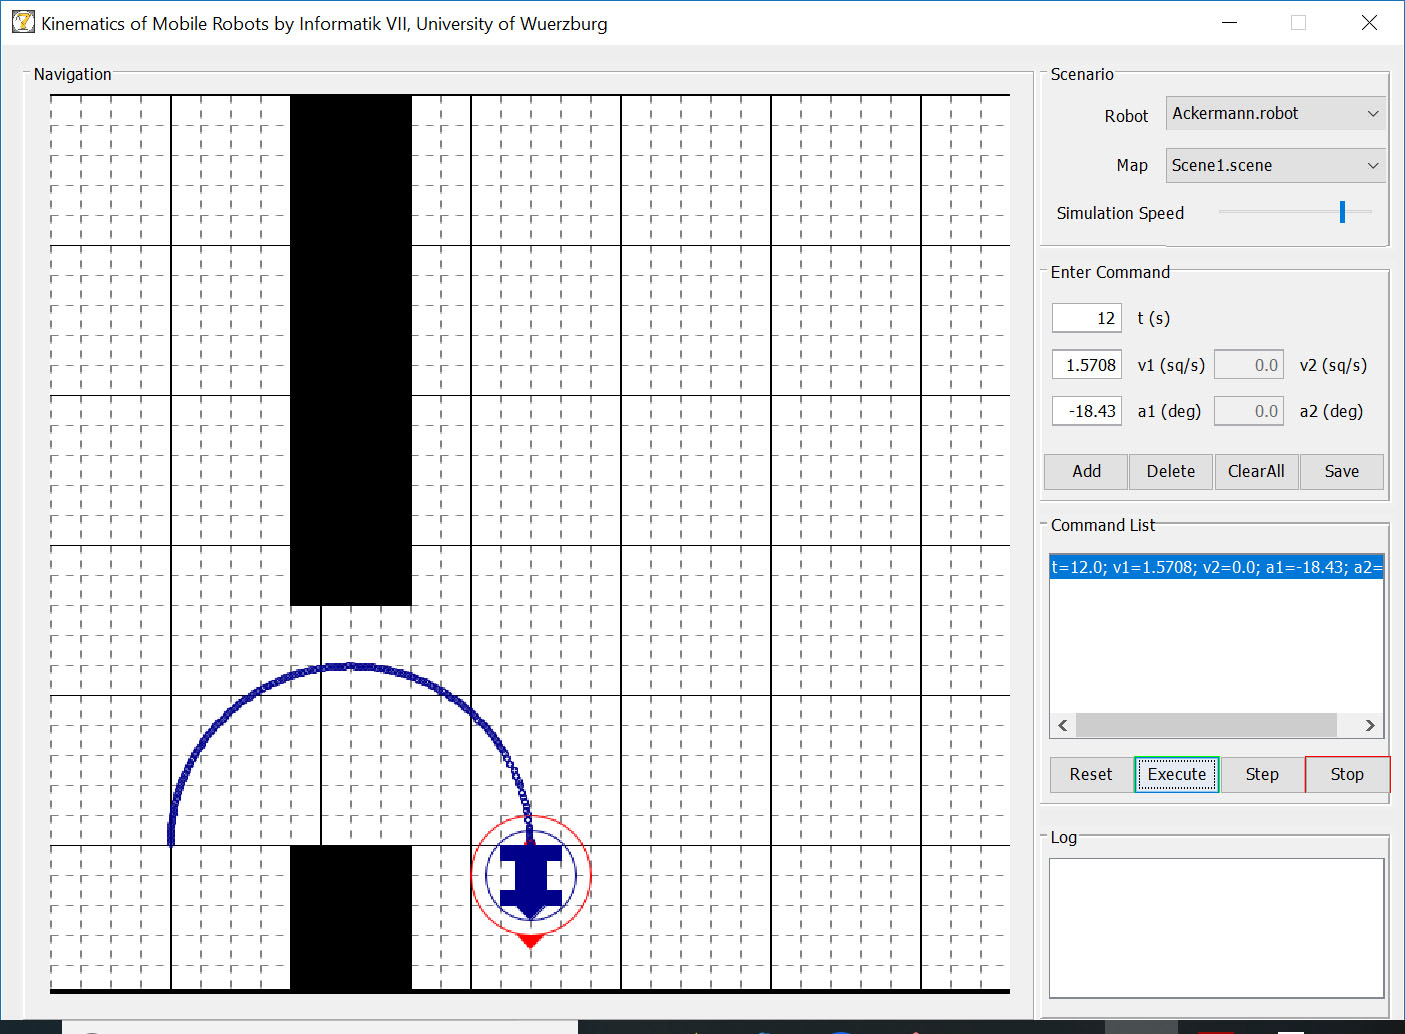
\includegraphics[width=0.8\textwidth]{figures/ackermann-scene-1.JPG}
	
	\paragraph{Ackermann robot - Scene 2} with the following maneuvers
	
	\begin{tabular}{|c|c|c|c|c|}
		\hline 
		$i$ & $t_i$ & $x(t_i)$ & $y(t_i)$ & $\theta(t_i)$ \\ 
		\hline 
		1 & 0 & 5 & 5 & $\frac{\pi}{2}$ \\ 
		\hline 
		2 & 6 & 11 & 11 & 0 \\ 
		\hline 
		3 & 12 & 17 & 17 & $\frac{\pi}{2}$ \\ 
		\hline 
		4 & 14 & 17 & 5 & $\frac{\pi}{2}$ \\ 
		\hline 
	\end{tabular} 
	\\

	\begin{gather}
	v_1 = \frac{(11-5)(0-\frac{\pi}{2})}{(6-0)(\sin(0) - \sin(\frac{\pi}{2})))} = \frac{\pi}{2} = 1,5708\\
	\varphi_1 = \arctan2(11 - 5, 2 (\sin(0) - \sin(\frac{\pi}{2}))) = -18.43^\circ\\
	v_2 = \frac{(17-11)(\frac{\pi}{2} - 0)}{(12-6)(\sin(\frac{\pi}{2}) - \sin(0)))} = \frac{\pi}{2} = 1,5708\\
	\varphi_2 = \arctan2(17 - 11, 2 (\sin(\frac{\pi}{2}) - \sin(0))) = 18.43^\circ\\
	v_3 = \frac{y(t_4) - y(t_3)}{t_4 - t_3} = -7
	\end{gather}\\
	$\varphi_3 = 0$ because the robot is already orientated correctly.\\
	\\
	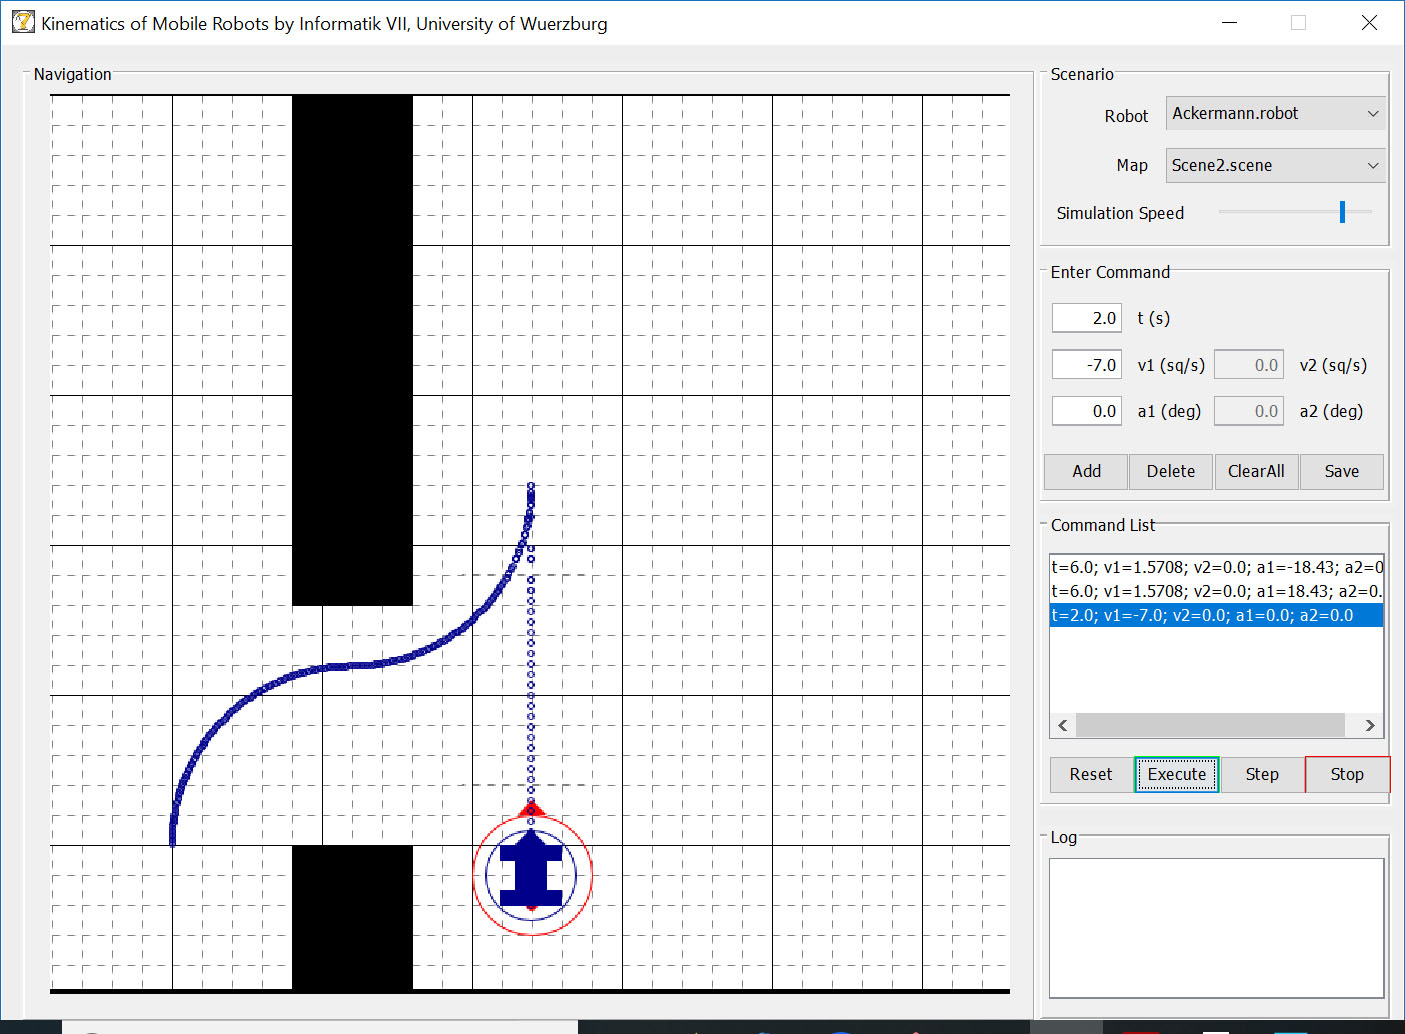
\includegraphics[width=0.8\textwidth]{figures/ackermann-scene-2.JPG}

\end{document}
